\documentclass[11pt,a4paper]{article}
% ============================================================
% Shared preamble for Claude Experiments reports (Ukrainian, LuaLaTeX)
% Compile with: lualatex report_*_uk.tex
% Include this AFTER \documentclass in each report:
%   \documentclass[11pt,a4paper]{article}
%   % ============================================================
% Shared preamble for Claude Experiments reports (Ukrainian, LuaLaTeX)
% Compile with: lualatex report_*_uk.tex
% Include this AFTER \documentclass in each report:
%   \documentclass[11pt,a4paper]{article}
%   % ============================================================
% Shared preamble for Claude Experiments reports (Ukrainian, LuaLaTeX)
% Compile with: lualatex report_*_uk.tex
% Include this AFTER \documentclass in each report:
%   \documentclass[11pt,a4paper]{article}
%   \input{../preamble_uk}
% ============================================================
% Cyrillic via LuaLaTeX + fontspec (pdflatex has no T2A here).
\usepackage{fontspec}
\setmainfont{DejaVu Serif}
\setsansfont{DejaVu Sans}
\setmonofont{DejaVu Sans Mono}
\usepackage[a4paper,top=2.5cm,bottom=2.5cm,left=2.5cm,right=2.5cm]{geometry}
\usepackage{amsmath,amssymb}
\usepackage{graphicx}
\usepackage{subcaption}
\usepackage{booktabs}
\usepackage{xcolor}
\usepackage[colorlinks=true,allcolors=blue]{hyperref}
\usepackage{microtype}
\usepackage{float}
\usepackage{array}
\microtypesetup{expansion=false}

% Color scheme
\definecolor{colMicro}{HTML}{222222}
\definecolor{colExact}{HTML}{2878b5}
\definecolor{colPlacement}{HTML}{e07a1f}
\definecolor{colBoundary}{HTML}{429c74}
\definecolor{colCurrent}{HTML}{c23b55}
\definecolor{colMM}{HTML}{c23b55}

\providecommand{\SIG}{\textcolor{green!50!black}{\textbf{*}}}
\providecommand{\NS}{\textcolor{gray}{n.s.}}
\providecommand{\DRMS}{\Delta\mathrm{RMST}}
\providecommand{\ci}[2]{$[{#1},\;{#2}]$}

% ============================================================
% Cyrillic via LuaLaTeX + fontspec (pdflatex has no T2A here).
\usepackage{fontspec}
\setmainfont{DejaVu Serif}
\setsansfont{DejaVu Sans}
\setmonofont{DejaVu Sans Mono}
\usepackage[a4paper,top=2.5cm,bottom=2.5cm,left=2.5cm,right=2.5cm]{geometry}
\usepackage{amsmath,amssymb}
\usepackage{graphicx}
\usepackage{subcaption}
\usepackage{booktabs}
\usepackage{xcolor}
\usepackage[colorlinks=true,allcolors=blue]{hyperref}
\usepackage{microtype}
\usepackage{float}
\usepackage{array}
\microtypesetup{expansion=false}

% Color scheme
\definecolor{colMicro}{HTML}{222222}
\definecolor{colExact}{HTML}{2878b5}
\definecolor{colPlacement}{HTML}{e07a1f}
\definecolor{colBoundary}{HTML}{429c74}
\definecolor{colCurrent}{HTML}{c23b55}
\definecolor{colMM}{HTML}{c23b55}

\providecommand{\SIG}{\textcolor{green!50!black}{\textbf{*}}}
\providecommand{\NS}{\textcolor{gray}{n.s.}}
\providecommand{\DRMS}{\Delta\mathrm{RMST}}
\providecommand{\ci}[2]{$[{#1},\;{#2}]$}

% ============================================================
% Cyrillic via LuaLaTeX + fontspec (pdflatex has no T2A here).
\usepackage{fontspec}
\setmainfont{DejaVu Serif}
\setsansfont{DejaVu Sans}
\setmonofont{DejaVu Sans Mono}
\usepackage[a4paper,top=2.5cm,bottom=2.5cm,left=2.5cm,right=2.5cm]{geometry}
\usepackage{amsmath,amssymb}
\usepackage{graphicx}
\usepackage{subcaption}
\usepackage{booktabs}
\usepackage{xcolor}
\usepackage[colorlinks=true,allcolors=blue]{hyperref}
\usepackage{microtype}
\usepackage{float}
\usepackage{array}
\microtypesetup{expansion=false}

% Color scheme
\definecolor{colMicro}{HTML}{222222}
\definecolor{colExact}{HTML}{2878b5}
\definecolor{colPlacement}{HTML}{e07a1f}
\definecolor{colBoundary}{HTML}{429c74}
\definecolor{colCurrent}{HTML}{c23b55}
\definecolor{colMM}{HTML}{c23b55}

\providecommand{\SIG}{\textcolor{green!50!black}{\textbf{*}}}
\providecommand{\NS}{\textcolor{gray}{n.s.}}
\providecommand{\DRMS}{\Delta\mathrm{RMST}}
\providecommand{\ci}[2]{$[{#1},\;{#2}]$}


\title{\textbf{Gateway separation audit: near, random і far architecture}\\[0.4em]
\large Структурна похибка двошарової апроксимації}
\author{Claude Experiments Series}
\date{7 серпня 2026}

\begin{document}
\sloppy
\maketitle

\begin{abstract}
У 100 парних мережевих блоках ($L=5$, $n=100$, $d=6$, $k=5$,
$\beta=0.003$, SI, $T_{\mathrm{end}}=2000$) термінальний restricted mean
MicroMacro був незмінним, 983.06, оскільки aggregate model не використовує
gateway identities. Натомість restricted mean Full Micro зріс від 905.42 для
near до 1265.17 для random і 1437.87 для far. Відповідно
$\Delta\mathrm{RMST}=\mathrm{MM}-\mathrm{Micro}$ змінив знак: $+77.64$,
$-282.11$ і $-454.81$. Парні контрасти random--near, far--near та far--random
мали 95\% CI, що не включали нуль. Однак політики одночасно змінювали
gateway separation, overlap і потенційні centrality properties, тому результат
ідентифікує ефект separation/overlap architecture, а не чистий distance-only
effect. Far оцінки є horizon-restricted через 4\% цензурування Full Micro.
\end{abstract}

\tableofcontents
\clearpage

\section{Статус і походження даних}\label{sec:status}

Повний експеримент завершено без failed replications: 100 парних мережевих
блоків, $L=5$, $n=100$, середній внутрішній ступінь $d=6$, $k=5$
міжспільнотних ребер, $\beta=0.003$, $\gamma=0$ (SI) та
$T_{\mathrm{end}}=2000$. Внутрішні графи й multiset внутрішніх ступенів
gateway-вузлів спарено між режимами. MicroMacro не використовує gateway
identities, тому його результат повторно використано для near, random і far
у межах реплікації. Збережено arrival times без траєкторій та event logs.

\section{Наукове питання}\label{sec:question}

Як архітектура вхідних і вихідних gateways усередині проміжної спільноти
змінює похибку двошарової апроксимації? Чи зростає розходження між Full Micro
та MicroMacro, коли export gateways обираються далі від gateways, через які
інфекція входить у спільноту?

\section{Дизайн та оцінювана величина}\label{sec:design}

У кожній із трьох проміжних спільнот фіксується left gateway set. Right set
із тим самим multiset внутрішніх ступенів обирається так:
\begin{description}
  \item[near] кандидати з найменшою відстанню до left set;
  \item[random] випадкові кандидати;
  \item[far] кандидати з найбільшою відстанню до left set.
\end{description}
Кількість bridge edges і всі внутрішні ребра незмінні. $D_{\min}$ і
$D_{\mathrm{mean}}$ --- середні за проміжними спільнотами мінімальна та
середня попарна відстань між left/right sets.

Для термінального шару
\[
 \begin{aligned}
 \Delta\mathrm{RMST}
   &=\mathrm{RMST}_{\mathrm{MicroMacro}}-\mathrm{RMST}_{\mathrm{Micro}},\\
 \Delta\mathrm{RMST}<0
   &\Longrightarrow \text{MicroMacro прибуває раніше}.
 \end{aligned}
\]
Неспостережені до горизонту прибуття замінено на $T_{\mathrm{end}}=2000$.
Тому всі середні, $W_1$ та міжрежимні contrasts є horizon-restricted.
Контрасти error ресемпловано за 100 paired network blocks.

\section{Кількісні результати}\label{sec:results}

\subsection{Gateway descriptors}

\begin{table}[H]
\centering
\caption{Відстань і overlap між left/right gateway sets. Знаменник 300 ---
три проміжні спільноти у кожній зі 100 реплікацій.}
\label{tab:descriptors}
\begin{tabular}{lrrr}
\toprule
Політика & $D_{\min}$ & $D_{\mathrm{mean}}$ & Комірки з overlap \\
\midrule
near   & 0.0000 & 2.2003 & 300/300 \\
random & 0.5567 & 2.6475 & 164/300 \\
far    & 1.9033 & 2.9892 & 24/300 \\
\bottomrule
\end{tabular}
\end{table}

$D_{\min}=0$ і overlap у 300/300 near-комірках показують, що near policy
систематично допускає спільні left/right gateway-вузли. Отже, табл.~\ref{tab:descriptors}
описує комплексну зміну архітектури, а не лише одного distance scalar.

\subsection{Термінальний шар}

MicroMacro має однаковий restricted mean 983.06 у всіх режимах.

\begin{table}[H]
\centering
\small
\caption{Термінальні horizon-restricted метрики на шарі 4.}
\label{tab:terminal}
\begin{tabular}{lrrrrr}
\toprule
Політика & Mean Micro & Comp. Micro & Comp. MM & $\Delta$RMST & rel-$W_1$ \\
\midrule
near   & 905.42  & 1.00 & 1.00 & $+77.64$  & 0.09235 \\
random & 1265.17 & 1.00 & 1.00 & $-282.11$ & 0.22298 \\
far    & 1437.87 & 0.96 & 1.00 & $-454.81$ & 0.31631 \\
\bottomrule
\end{tabular}
\end{table}

Для far значення 1437.87 і $-454.81$ у табл.~\ref{tab:terminal} restricted
до 2000: чотири незавершені Micro-прогони мають внесок 2000. Уже в шарі 3
completion Micro для far дорівнює 0.99, тоді як MicroMacro --- 1.00. У шарі 1
результати збігаються між політиками, бо endpoint gateway sets не змінювалися.

\subsection{Парні міжрежимні контрасти}

\begin{table}[H]
\centering
\caption{Різниці термінального error між gateway policies; bootstrap unit ---
paired network block.}
\label{tab:contrasts}
\begin{tabular}{lrr}
\toprule
Контраст error & Оцінка & 95\% CI \\
\midrule
random $-$ near & $-359.74$ & $[-413.68,-305.50]$ \\
far $-$ near    & $-532.45$ & $[-586.68,-478.01]$ \\
far $-$ random  & $-172.70$ & $[-230.57,-114.84]$ \\
\bottomrule
\end{tabular}
\end{table}

Усі CI в табл.~\ref{tab:contrasts} не включають нуль у цьому наборі.
Зі зміною architecture від near до far Full Micro прибуває пізніше, тоді як
MicroMacro залишається незмінним, тому error стає більш від'ємним.

\subsection{Графічне резюме}

\begin{figure}[H]
  \centering
  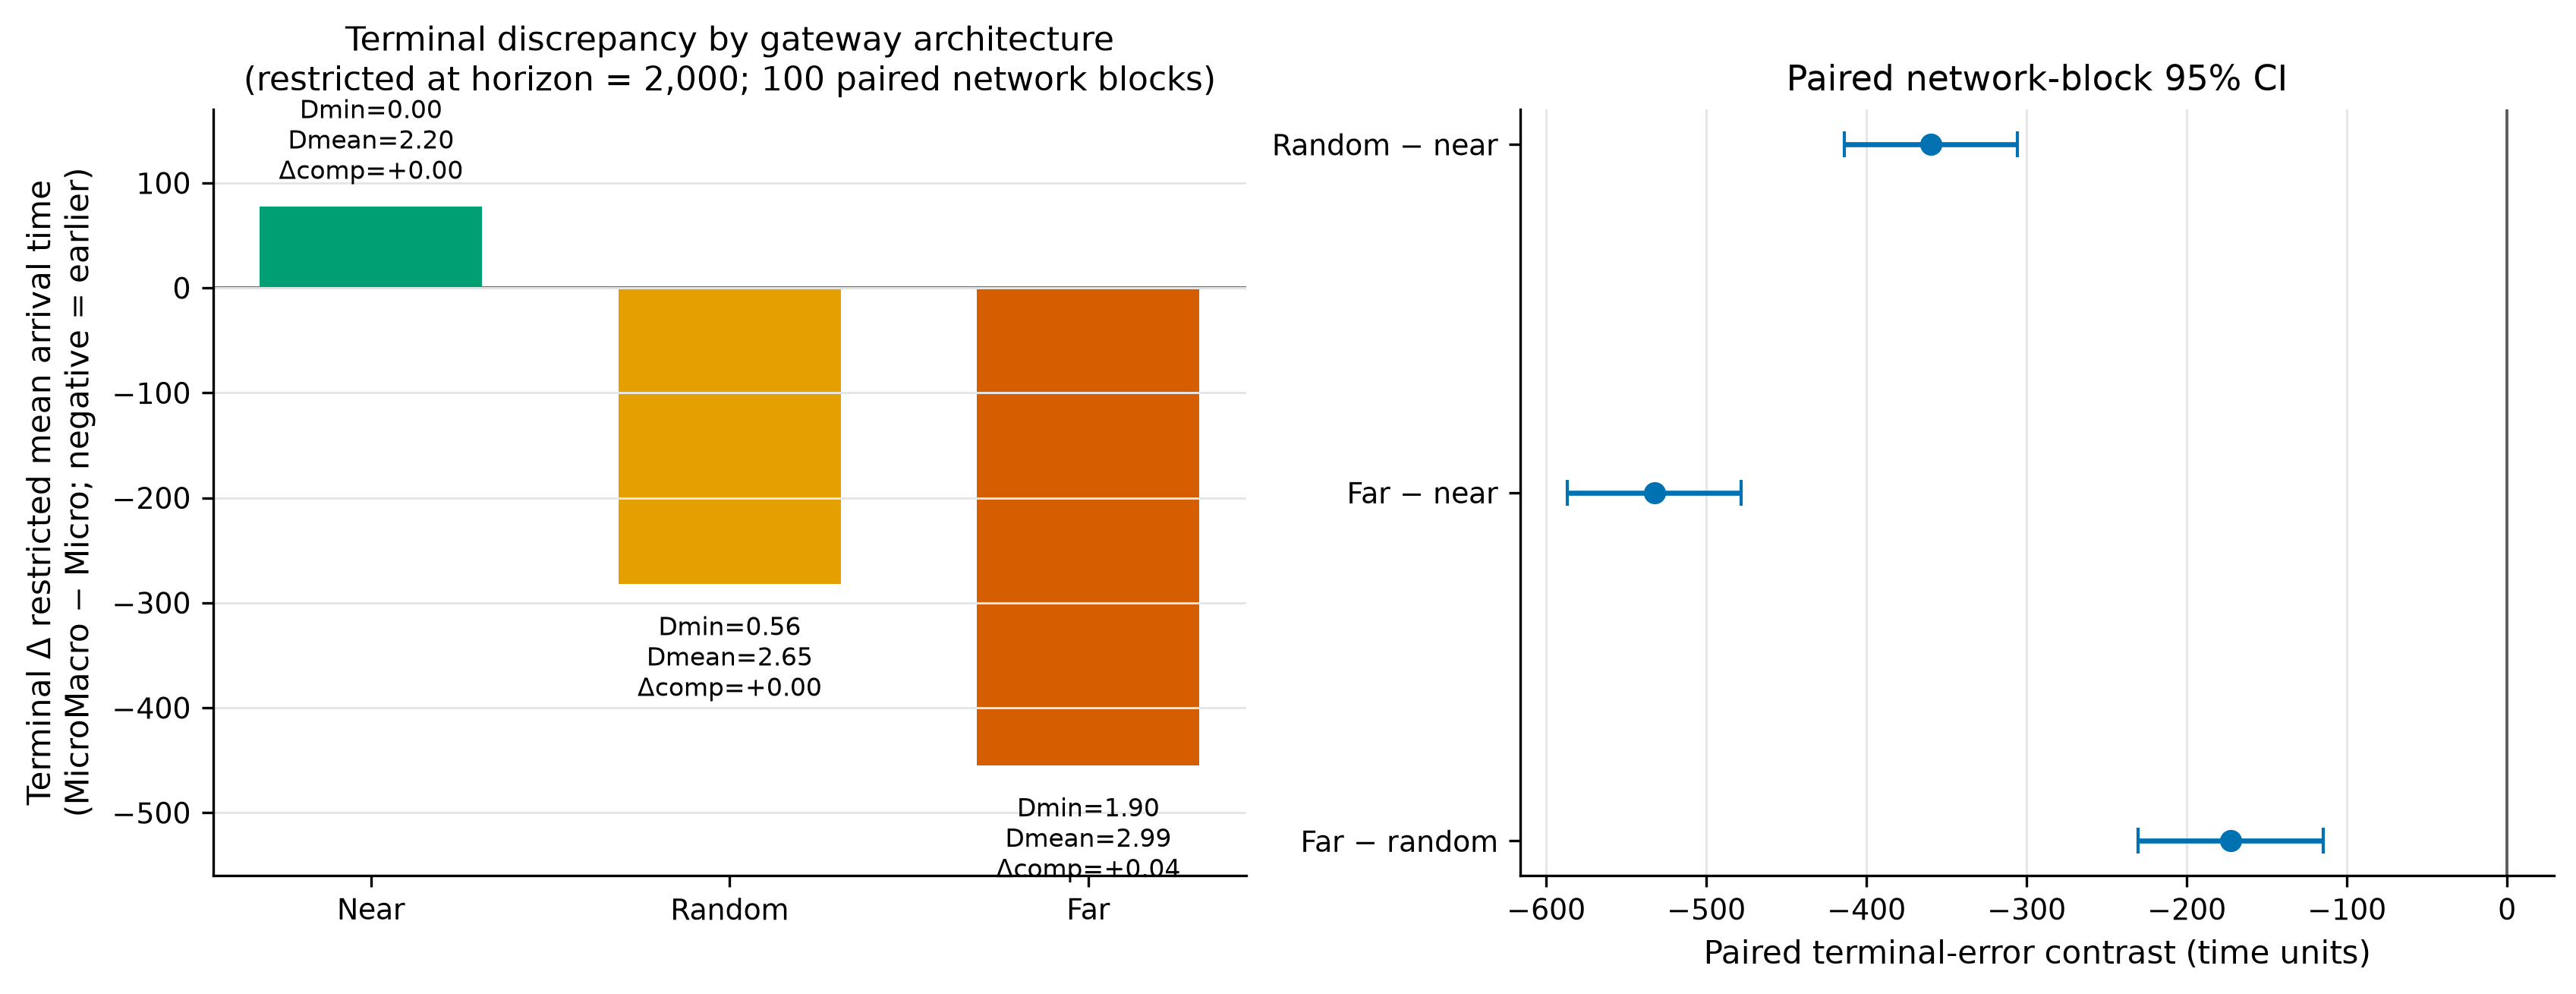
\includegraphics[width=0.94\linewidth]{figures/report_figure.png}
  \caption{Gateway descriptors, terminal approximation error і paired
  міжрежимні контрасти. Far оцінки слід читати як restricted до 2000 через
  цензурування, наведене в табл.~\ref{tab:terminal}.}
  \label{fig:gateway}
\end{figure}

\section{Аналіз та каузальна інтерпретація}\label{sec:interpretation}

Однакові community counts і матриця $W$ не кодують, наскільки легко інфекція
проходить від import до export gateways усередині спільноти. Near architecture
дає коротший шлях і часто повторно використовує ті самі вузли; far architecture
вимагає більшого внутрішнього поширення до наступного export. MicroMacro не
розрізняє ці випадки, тому його terminal mean незмінний.

Парування внутрішніх графів, кількості bridge edges і within-degree multiset
усуває важливі confounds. Проте policies різко змінюють overlap і можуть
змінювати centrality та інші позиційні властивості. Тому causal treatment слід
називати \emph{gateway separation/overlap architecture}, а не чистим
distance-only effect.

Зміна знаку в табл.~\ref{tab:terminal} є принциповою: одна aggregate
параметризація може запізнюватися в near ($+77.64$) та випереджати Full Micro
у random/far. Отже, знак approximation bias не є інваріантним до прихованої
мезоскопічної gateway geometry. Рис.~\ref{fig:gateway} візуалізує цей
структурний stress test, але не усуває overlap confounding.

\section{Значення для двошарової апроксимації та статті}\label{sec:paper}

\begin{itemize}
  \item Community-level edge counts недостатньо для прогнозу arrival-time
  error за змінної import/export architecture.
  \item Gateway geometry є джерелом rate-abstraction error: aggregate hazard
  не враховує час досягнення export boundary.
  \item Bridge-aware модель може потребувати стану export-gateway availability
  або crossing-delay surrogate.
  \item Експеримент слід подавати як paired structural stress test, а не як
  універсальну монотонну залежність від graph distance.
\end{itemize}

\section{Обмеження і твердження, яких слід уникати}\label{sec:limits}

\begin{enumerate}
  \item Far terminal results мають 4\% цензурування Micro і чинні лише як
  restricted-at-2000 estimands. Їх не можна прирівнювати до необмеженого mean.
  \item Overlap і потенційні centrality differences не контрольовано окремо;
  чистий ефект відстані не ідентифіковано.
  \item Перевірено одну SI-конфігурацію, connected ER-like graphs, $L=5$ і
  $k=5$; переносимість на SIR та інші топології не встановлено.
  \item rel-$W_1$ і $\Delta\mathrm{RMST}$ описують різні аспекти розподілу.
  \item Bootstrap CI в табл.~\ref{tab:contrasts} стосуються міжрежимних
  contrasts, а не окремих $\Delta\mathrm{RMST}$ у табл.~\ref{tab:terminal}.
  \item Експеримент не оцінює runtime і не підтримує тверджень про прискорення.
\end{enumerate}

\section{Практичні рекомендації}\label{sec:recommendations}

\begin{enumerate}
  \item У наступному дизайні зробити gateway sets disjoint у всіх режимах або
  факторизувати overlap і distance окремо.
  \item Match/record centrality, distance quantiles і час першого зараження
  export gateway для механістичного аналізу crossing delay.
  \item Для far використати довший або наперед спільно зафіксований горизонт
  і survival/RMST analysis; не аналізувати лише completed arrivals.
  \item Калібрувати bridge-aware state на layerwise error і перевіряти зміну
  знаку bias.
\end{enumerate}

\section{Відтворення}\label{sec:reproduction}

Runner: \path{extrascripts/run_gateway_distance_sweep.py}. \\
Зведені результати: \path{output/missing_experiments/gateway_distance/full/summary.csv}
і \path{output/missing_experiments/gateway_distance/full/contrasts.csv}. \\
Реплікаційні записи: \path{output/missing_experiments/gateway_distance/full/replications/}. \\
Маніфест: \path{output/missing_experiments/gateway_distance/full/manifest.json}.
Він фіксує config fingerprint, параметри, seed policy, pairing і статус усіх
100 реплікацій.

\end{document}
